\documentclass{article}
\usepackage[utf8]{inputenc}
\usepackage[russian]{babel}
\usepackage{amsmath}

\begin{document}

\section{Часть 1}

\subsubsection{Суть игрового процесса}
Игровой процесс в данной игре представляет собой захватывающее сочетание платформера и стратегии, где игроку предстоит пройти через пять уникальных уровней, каждый из которых соответствует различным аспектам учебной программы «Компьютерные науки и технологии». Игрок берет на себя роль студента, который сталкивается с агрессивными врагами, представляющими собой дисциплины, предметы и приложения, стремящиеся помешать его успеваемости.\par
Основные элементы игрового процесса:\par
\begin{enumerate}
    \item \textbf{Платформенные элементы} \par
    Игроку предстоит прыгать, избегать препятствий и сражаться с врагами, используя свою ловкость и внимательность. Прыжки сверху на врагов — ключевой способ их уничтожения.
    \item \textbf{Стратегия и выбор пути} \par
    Игрок должен разрабатывать свою стратегию на каждом уровне, выбирая наиболее эффективный путь для достижения цели. Это включает в себя анализ препятствий и врагов, а также принятие решений о том, как лучше всего использовать свои навыки.
    \item \textbf{Система оценок} \par
    За успешное преодоление уровней и уничтожение врагов игрок получает «десятки», которые служат не только для прохождения на следующий уровень, но и как символ успеха и знаний игрока.
    \item \textbf{Разнообразие врагов и препятствий} \par
    Каждый уровень предлагает уникальных врагов и препятствий, что делает игровой процесс разнообразным и увлекательным. Игрок сталкивается с различными тактиками и подходами для победы над каждым видом противника.
\end{enumerate}
Игрок получает удовольствие от сочетания динамичного игрового процесса, стратегического мышления и возможности видеть свой прогресс.

\section{Часть 2}

\subsection*{Персонаж игрока}

\begin{itemize}
    \item \textbf{Персонаж игрока - студент Высшей школы экономики} \\ 
    Данный персонаж - добрый, замотированный в учебе и преодолении различных сложностей во время учебного процесса студент. Он готов справляться с ними во что бы то ни стало и не опускать руки. На персонаже футболка из мерча Высшей школы экономики с надписью "HSE" для поддержания корпоративного стиля ВУЗа. В качестве цвета футболки выбран синий - самый узнаваемый цвет из брендбука ВШЭ, с которым знаком каждый студент Вышки. 
\end{itemize}

\section{Часть 3}

\subsection*{Элементы игры}

Игра представляет из себя платформер с элементами roguelike — это жанр компьютерных игр, который сочетает в себе элементы двух жанров: платформера и roguelike.

\begin{enumerate}
    \item \textbf{Противники} \par
    На каждом уровне игрок сталкивается с уникальными врагами, которые требуют разных подходов для победы над ними.
    Противники подразделяются на классы:
    \begin{itemize}
        \item \textbf{Противники ближнего боя:} \par
        Итеграл, философия
        \item \textbf{Противники дальнего боя:} \par
        SmartLMS, python, ворона, Яндекс.Почта
        \item \textbf{Боссы:} \par
        Диплом
    \end{itemize}
    Каждый из этих противников олицетворяет собой одну из трудностей, с которыми сталкиваются студенты Высшей школы экономики на пути к выпуску.
    \item \textbf{Уровни} \par
    Каждый уровень представляет собой отдельный курс обучения. Игра состоит из пяти уровней, и на каждом из них игрока ждут разнообразные противники и уникальное расположение игровых элементов.
    \item \textbf{Игровые элементы} \par
    \begin{itemize}
        \item Препятствия, ловушки
        \item Платформы, являющиеся основной составляющей уровней.
    \end{itemize}
    \item \textbf{Сложность} \par
    С каждым уровнем сложность игры повышается, а поведение врагов становится более непредсказуемым. Это заставляет игрока постоянно осваивать новые игровые механики, что поддерживает интерес к игре.
\end{enumerate}

\section{Часть 4}

\subsection*{Физическая модель}

\begin{itemize}
    \item \textbf{Физическая модель игрового мира} \par
    Физическая модель игрового мира базируется на упрощенной физике, которая делает управление персонажем интуитивно понятным и отзывчивым для игрока. Основные законы физики такие, как гравитация и т.п., адаптированы для создания ощущения плавного и предсказуемого взаимодействия между персонажем, объектами и окружением.
    \item \textbf{Перемещение} \par
    Персонаж может перемещаться влево или вправо с постоянной максимальной скоростью, достигая её плавно (ускорение). Также, как и почти во всех играх такого типа, реализована механика прыжков, которые подчиняются параболической траектории и высотой которых можно управлять с помощью зажатия клавиши прыжка.
    \item \textbf{Боевые действия} \par
    Прыжок сверху на врага — это базовая атака, которая уничтожает или обезвреживает большинство врагов. Это ключевая механика, которая является простой для освоения, но при этом может быть достаточно сложной в реализации для определенных противников.
\end{itemize}

\section{Часть 5}

\subsection*{Искусственный интеллект}

Искусственный интеллект (AI) в игре разработан так, чтобы создавать атмосферу, отражающую реальные студенческие трудности, при этом оставаясь простым и понятным для игрока.

\textbf{Общие принципы поведения AI:}

\begin{enumerate}
    \item \textbf{Противники ближнего боя:}  
    Эти враги, такие как интеграл или значок Яндекс.Почты, патрулируют ограниченные территории. Если игрок попадает в зону их действия, они начинают преследование. При уходе игрока за пределы зоны враги возвращаются к своему маршруту.  

    \item \textbf{Противники дальнего боя:}  
    Например, <<-10>> или философия. Эти враги атакуют, если игрок оказывается в их зоне видимости. Они фиксируются на игроке до тех пор, пока он не укрывается или не выходит за пределы зоны атаки.  

    \item \textbf{Летающие противники:}  
    Такие как вышкинская ворона или SmartLMS. Эти враги двигаются по заданной траектории, периодически стреляя в игрока. Если игрок долго находится в их зоне, враги могут начать его преследовать.  

    \item \textbf{Поведение на уровнях:}  
    \begin{itemize}
        \item На первых уровнях враги действуют просто: патрулируют или атакуют игрока при входе в зону действия.  
        \item На более сложных уровнях враги могут действовать координированно, усиливая давление на игрока. Например, ближние и дальние противники могут перекрывать пути отхода.  
    \end{itemize}
    \item \textbf{Эмоциональный эффект:}  
    \begin{itemize}
        \item AI создаёт умеренный вызов для игрока, поддерживая атмосферу игры.  
        \item Противники не только атакуют, но и добавляют комичные элементы, например, ироничные фразы или необычное поведение, что делает игровой процесс более увлекательным.  
    \end{itemize}
\end{enumerate}

\section{Часть 6}

\subsection*{Интерфейс пользователя}
\begin{itemize}
    \item \textbf{Схема навигации по по меню игрового интерфейса и оболочки игры} \\
   \begin{figure}[h]
    \centering
    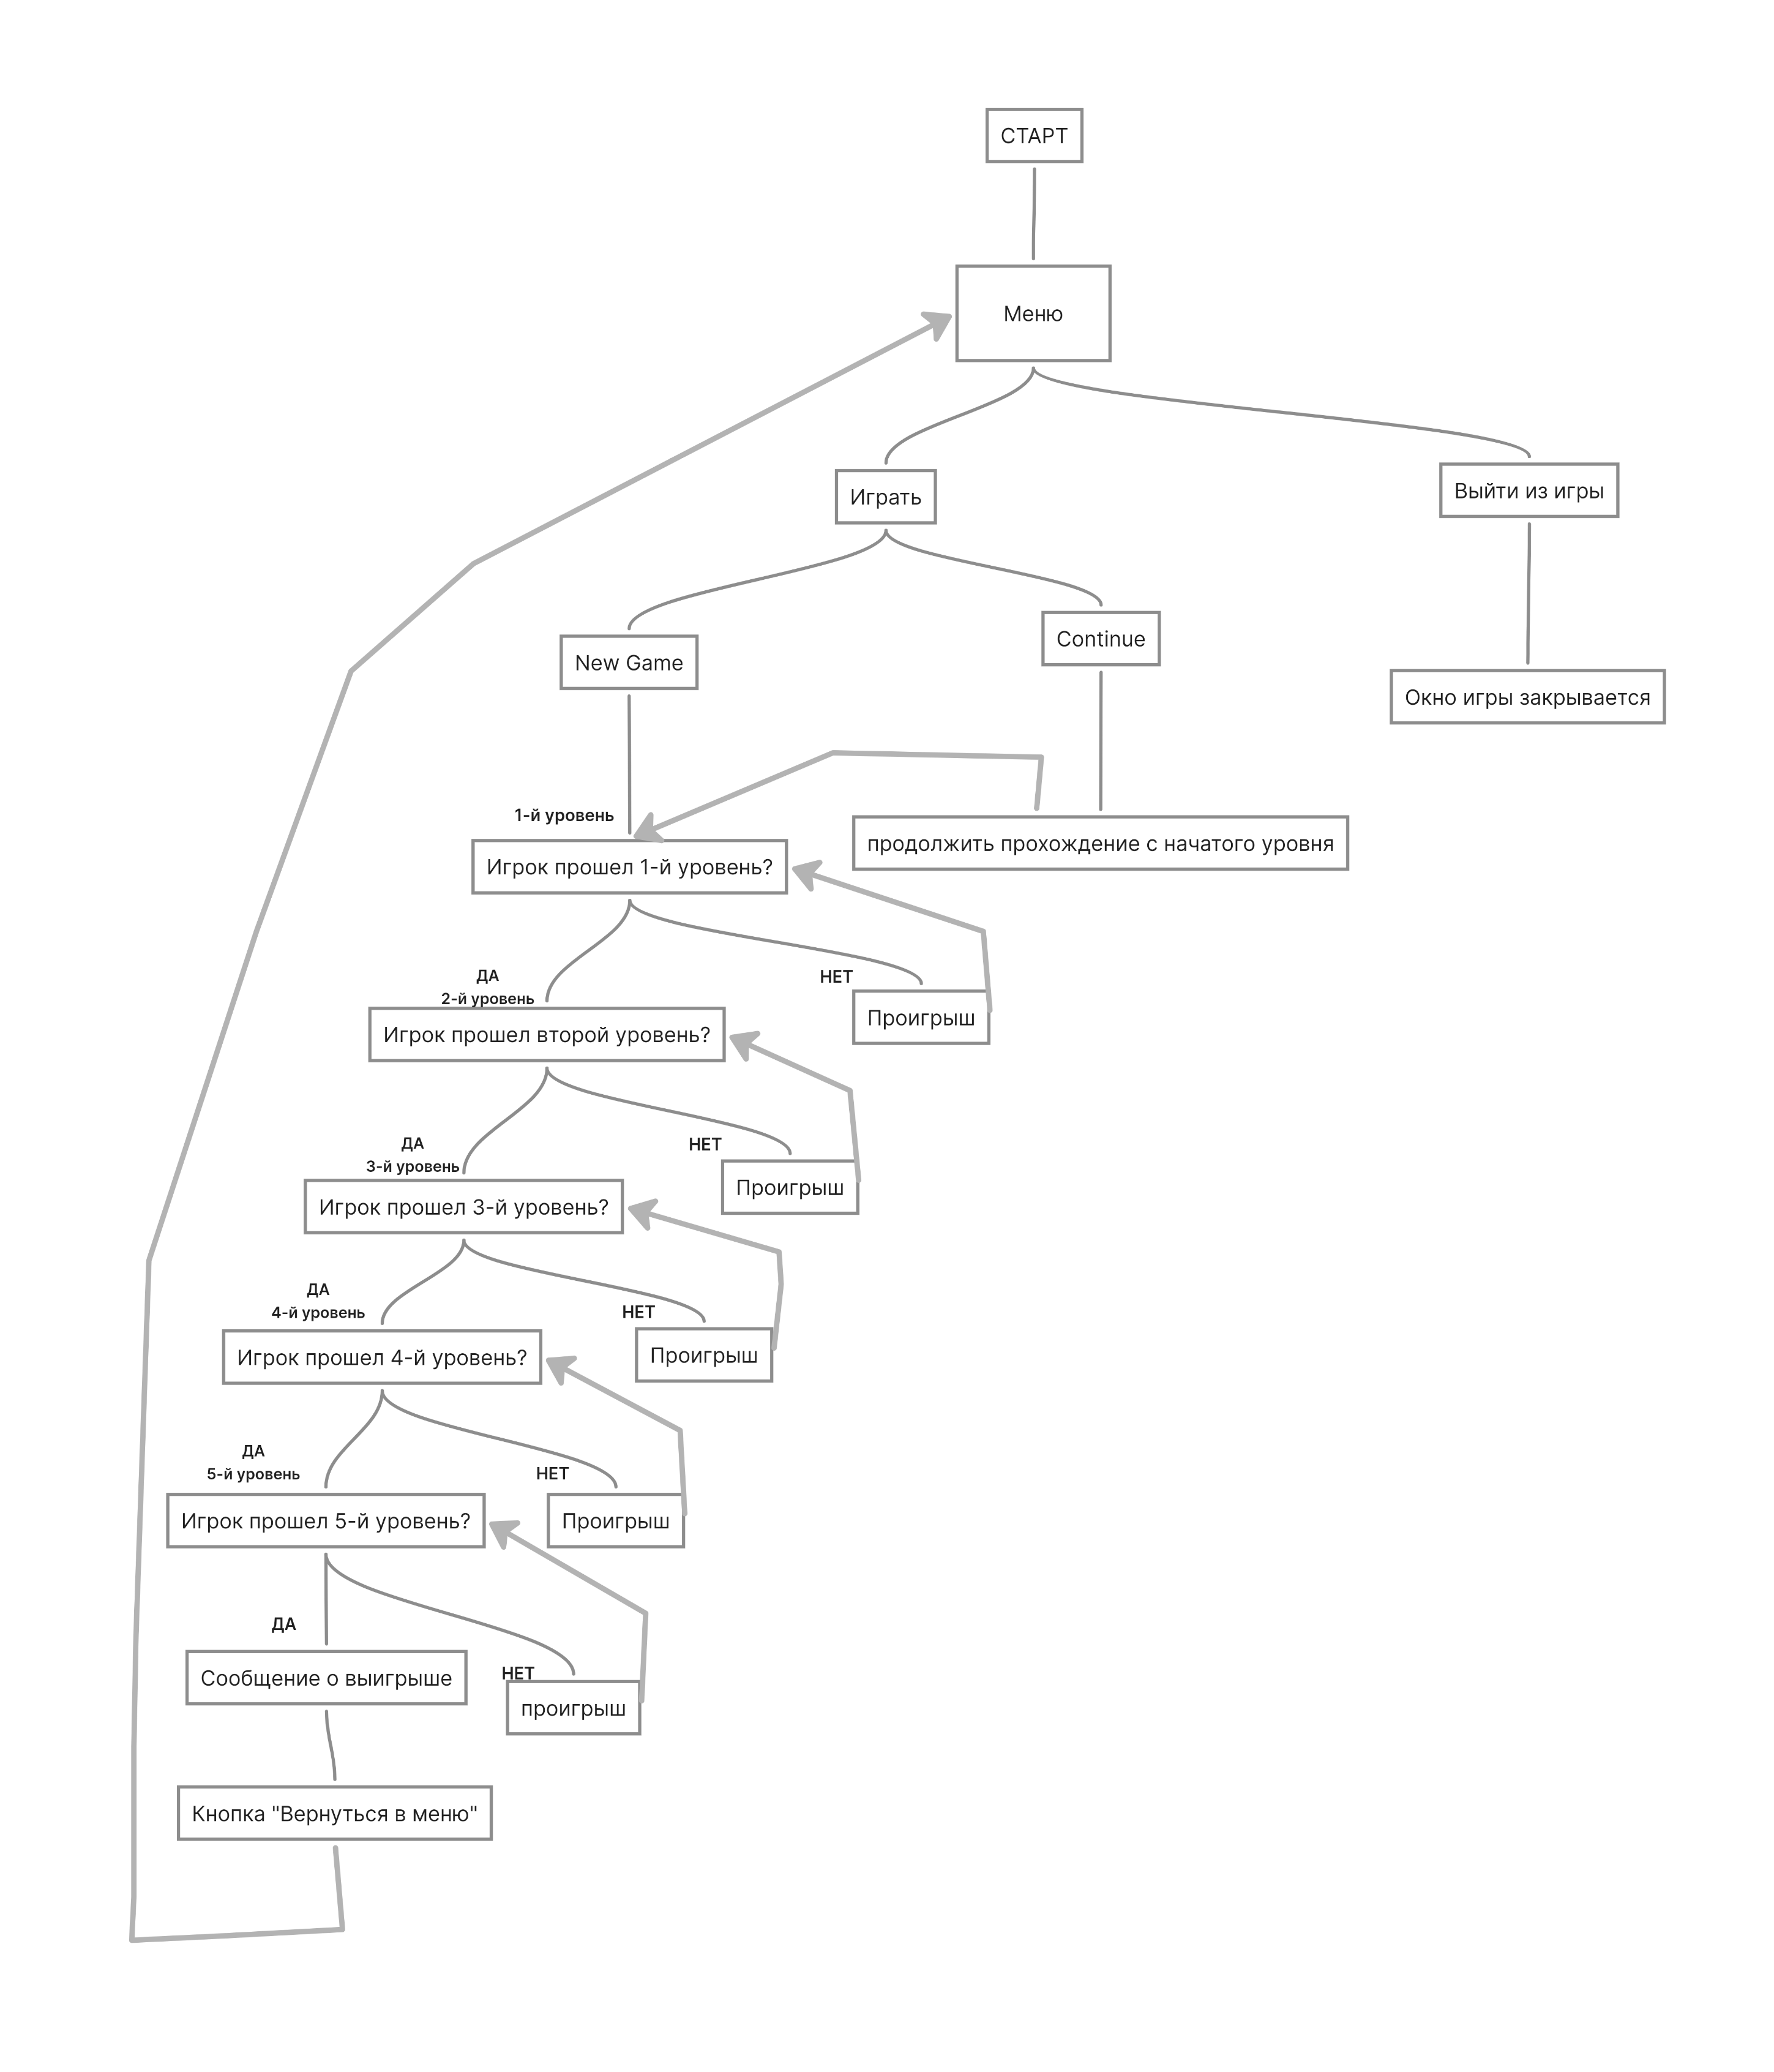
\includegraphics[width=1.0\linewidth]{схема.png}
    \caption{Блок-схема игры-платформера "HSE" на Unity}
    \label{fig:mpr}
    \end{figure}
\end{itemize}

\subsection*{Функциональное описание и управление}
Функциональный интерфейс состоит из следующих экранов:
\begin{enumerate}
  \item \textbf{Экран меню} \par
      Предоставляет пользователю интерфейс для управления игровым процессом. Позволяет начинать игру, запускать с последнего сохранения, завершать игру с последующим выходом.
  \item \textbf{Экран игрового процесса} \par
      Предоставляет пользователю интерфейс для взаимодействия с игровым процеесом. Позволяет управлять персонажем, взаимодействовать с игровым окружением, возвращаться в главное меню.
  \item \textbf{Финальный экран}\par
      Информирует пользователя об успешном прохождении игры и предоставляет интерфейс для выхода в меню.
\end{enumerate}

\subsection*{Объекты интерфейса пользователя}

\begin{enumerate}
    \item \textbf{Кнопки в главном меню:}  
    Главный экран содержит следующие кнопки:  
    \begin{itemize}
        \item \textbf{Начать игру:} запускает новую игру с самого начала.  
        \item \textbf{Продолжить:} загружает последнее сохранение.  
        \item \textbf{Выход:} завершает игру и закрывает приложение.  
    \end{itemize}

    \item \textbf{Кнопки на каждом уровне:}  
    На каждом уровне в правом верхнем углу экрана отображается кнопка:  
    \begin{itemize}
        \item \textbf{Возврат в главное меню:} позволяет игроку выйти из текущего уровня и вернуться в главное меню. При нажатии на эту кнопку прогресс текущего уровня не сохраняется.  
    \end{itemize}

    \item \textbf{Финальный экран:}  
    После завершения игры появляется простой экран с текстом, уведомляющим игрока об окончании игры.  
    \begin{itemize}
        \item \textbf{Кнопка возврата в меню:} позволяет игроку вернуться в главное меню для повторного прохождения или выхода из игры.  
    \end{itemize}
\end{enumerate}

\section{Часть 7}

\subsection*{Графика и видео}
Раздел описывает характер и состав визуальной части игры, элементов игрового процесса

\subsection*{Общее описание}
    \begin{enumerate}
    \item \textbf{Техническое исполнение} \par
    Графика игры выполнена в 2D формате. В игре детально проработаны модели и анимации персонажей, так как каждый элемент игры отрисован вручную. Использование векторной графики позволило сделать линии более чёткими и масштабировать модели без потери качества.
    \item\textbf{Стилистика, атмосфера и палитра} \par
    Графический стиль игры базируется на карикатурной идее, поэтому игра ощущается легко и позитивно. Яркий и насыщенный белый фон влекёт за собою внимание и погружает игрока в живую среду студента Вышки. А на контрасте с тёмным кирпичом даёт понять игроку, что путь его ждёт не простой. Анимации персонажей усиливают чувство динамичности игры.
    \item \textbf{Другие общие сведения} \par
    Графика в игре сочетает в себе элементы платформера и стратегии. Сочетание платформера и стратегии в графическом исполнении однозначно придаёт проекту уникальности и разнообразия. Визуальные элементы платформера, такие как блочные структуры и препятствия, чётко выделены и легко воспринимаются. Это позволяет игрокам быстро ориентироваться в пространстве и строить стратегии для преодоления препятствий. Анимации врагов и персонажей проработаны таким образом, чтобы игрок мог предугадывать их действия. Динамичность анимации делает игру более захватывающей — сражения с врагами превращаются в живое представление.
    \end{enumerate}

\subsection*{Двумерная графика}
В данном разделе описана основная 2D графика и анимация, которые необходимо разработать для игры.
\begin{enumerate}
  \item \textbf{Интерфейс} \par
  В игре реализовано меню с возможностью начать новую игру или продолжить с того места, где игрок остановился. Также предусмотрена опция выхода из игры с автосохранением. Интерфейс выполнен в минималистичном, но интуитивно понятном стиле. Управление персонажем осуществляется с помощью клавиш \texttt{WASD} или стрелок на клавиатуре, взаимодействие с меню — через курсор мыши.
  \item \textbf{Эффекты} \par
  При уничтожении врагов происходит эффект их мгновенного исчезновения. Также при попадании снарядов противника в игрока, тот моментально выводится из игры, что сопровождается визуальным эффектом.
  \item \textbf{Персонажи, строения и юниты} \par
  Для моделей персонажей, противников и уровней использована векторная графика. Нарисовано: 1 главный герой, 12 различных противников, 1 босс, блоки для генерации уровня и фоновая заставка. Персонаж имеет анимацию передвижения и прыжков.
  \item \textbf{Игровой мир} \par
  Игровой мир выполнен в светлых тонах: стены корпуса Вышки имеют белый цвет, а пол и потолок — тёмные оттенки кирпича.
\end{enumerate}

\end{document}

